
\chapter{The Language}

\par The MalbolgeLISP implements a Lisp dialect which is described in this chapter. The main differences from Lisp is emphasis on functional programming, immutability and minimisation of the state (MalbolgeLISP doesn't implement \verb|setcar!| or \verb|setcdr!|). MalbolgeLISP borrows it's core features from Scheme, Haskell and APL, while using Lisp as a foundation or framework for constructing a language.

\section{Arithmetic}

\par MalbolgeLISP supports the following arithmetic operations:

\begin{itemize}
    \item \verb|+|, \verb|+'| - unsigned bounded addition\footnote{obeying to the laws of modular arithmetic; the result is truncated to 26 bits} and unbounded addition\footnote{on standards-compliant interpreters}
    \item \verb|-|. \verb|-'| - unsigned bounded subtraction and unbounded subtraction.
    \item \verb|*|, \verb|/|, \verb|%| - unsigned bounded multiplication, division and modulus.
    \item \verb|~| - boolean negation - $f(x) = 0$ for $x > 0$ and $f(x) = 1$ otherwise.
    \item \verb|!| - factorial function - $f(x) = x!$ computed using a lookup table for $x \leq 11$ and $f(x) = 0$ otherwise, since $!12$ exceeds the word size.
    \item \verb|^| - $n$-th power function assuming $0^0=1$.
    \item \verb|&| - logical AND function - $f(x, y) = 1$ for $x > 0 \wedge y > 0$, $f(x, y) = 0$ otherwise.
    \item \verb=|= - logical AND function - $f(x, y) = 0$ for $x = 0 \wedge y = 0$, $f(x, y) = 1$ otherwise.
    \item \verb|=|, \verb|/=| - equality and inequality.
    \item \verb|<|, \verb|>|, \verb|<=|, \verb|>=| - correspondingly: lesser than, greater than, lesser or equal to, greater or equal to.
    \item \verb|gcd|, \verb|lcm| - greatest common divisor and least common multiple.
    \item \verb|min|, \verb|max| - pick the smaller or larger value (\textit{minimum} or \textit{maximum}).
\end{itemize}

\par Demonstration of the arithmetic functions follows:

\begin{verbatim}
% (+ 2 1)
..............|.....
3
% (* 3 3)
..............|.....
9
% (% 5 2)
..............|.....
1
% (> 5 6)
..............|.....
0
% (< 5 6)
..............|.....
1
% (= 6 6)
..............|......
1
% (= (~ (= 6 7)) (/= 6 7))
......................|.........
1
% (/ 25 5)
..............|.....
5
% (- 4 3)
..............|.....
1
% (& (= 2 2) (= 3 3))
....................................|...............
1
% (| (= 2 3) (= 3 2))
................|..........
0
% (lcm 14 29)
......|....
406
% (max 5 (max 8 10))
...........|.......
10
% (^ 2 8)
......|....
256
% (! 6)
.....|...
720
\end{verbatim}

\section{Conditional execution}

\par In MalbolgeLISP, conditional evaluation is accomplished using \verb|if| and \verb|cond|\footnote{also \verb|iterate|, \verb|iterateN|, etc..., but these functions weren't designed for conditional evaluation and it only happened so that they can be used for this purpose, so they won't be covered in this section.}. \verb|&| and \verb=|= don't short-circuit, meaning that their operands are always evaluated. \verb|if| is very similar in it's structure to \verb|if..else| statements\footnote{or ternary operator expressions} known from languages like C++ or Java - \verb|(if condition valueIfTrue valueIfFalse)|. The short-circuiting aspect of \verb|if| can be demonstrated - If both cases of the \verb|if| condition were evaluated, the interpreter would print \verb|yes| and \verb|no| before yielding the correct result:

\begin{verbatim}
% (def noisy_eq (dyad (if (= x y) (print yes) (print no))))
.............................|..
(lambda (x y) (if (= x y) (print yes) (print no)))
% (noisy_eq 5 6)
......|............
no

no
% (noisy_eq 6 6)
......|............
yes

yes
\end{verbatim}

\par The \verb|cond| function is essentially a chain of \verb|if| expressions. To demonstrate the convenience of using \verb|cond| over multiple \verb|if| expressions, two implementations of three-way comparison are given:

\begin{verbatim}
; An implementation that uses if.
% (def <=> (dyad (
    if (= x y) eq (
        if (> x y) gt (
            if (< x y) lt unreachable)))))
...........................................|..
(lambda (x y) (if (= x y) eq (if (> x y) gt (if (< x y) lt unreachable))))
% (<=> 5 5)
......|..........
eq
% (<=> 6 7)
......|....................
lt
% (<=> 7 6)
......|...............
gt

; An implementation that uses cond.
% (def <=> (dyad (cond
    ((= x y) eq)
    ((> x y) gt)
    ((< x y) lt)
    (unreachable))))
...............................................|..
(lambda (x y) (cond ((= x y) eq) ((> x y) gt) ((< x y) lt) (unreachable)))
% (<=> 6 6)
......|...........
eq
% (<=> 6 7)
......|...................
lt
% (<=> 7 6)
......|...............
\end{verbatim}

\par It's worth mentioning that an \verb|if| expression must include a truthy and falsy clause (since the expression must evaluate to something and it's impossible to guarantee that the condition is always true). This isn't the case with the \verb|cond| expression. If one is certain that a \verb|cond| expression is already exhaustive, it doesn't have to provide a default case. The interpreter will error if the \verb|cond| expression isn't exhaustive and no default case was provided, though.

\section{Let bindings and the scope}

\par In MalbolgeLISP, there is a single way to bind variables without scope (via macros), and two ways of binding lexically scoped variables. Variables are usually bound using \verb|lambda| and all the covers over it (\verb|dyad|, \verb|monad|, \verb|defun|), but there is a way to bind variables without explicitly using a lambda expression - \verb|let| bindings. \verb|let| accepts a list of atoms to be bound interleaved with their values and the code to execute in the freshly created scope. The main difference from \verb|let| present in other lisps is that the binding list is flattened:

\begin{verbatim}
% (let (x 5 y 6) (print [x + y]))
.....................|............
11

11
\end{verbatim}

\par When evaluated, \verb|let| is desugared to a lambda expression with reversed parameters. The conversion schema follows:

\begin{verbatim}
(let (x x0 y y0 z z0 ...) (...)) => ((lambda (z y x ...) (...)) z0 y0 x0 ...)
\end{verbatim}

\par The real parameter order is reversed, since the interpreter (for the sake of simplicity) iterates over the input list and uses \verb|cons| to create the resulting desugared expression. Single-variable \verb|let| bindings could illustratively also be implemented as a macro:

\begin{verbatim}
% (defmacro let' (x y c) ((lambda (x) (eval c)) y)))
............................|.
macro/syn
% (let' x 5 (print x))
...........|...........
5

5
\end{verbatim}

\par The current scope is bound to the lambda expression at the time of it's creation. Since lazily evaluated values utilise closures which are lexically scoped, this property applies to them as well. Consequently, everything inside the lazily evaluated expression has access to the lexical ancestor's bound variables. Generally speaking, the global scope can be modified using \verb|def|, \verb|defun| and \verb|defmacro|, regardless of where these functions appear. Modifying the local scope is possible using only lambda expressions and the \verb|let| function. It's discouraged to use \verb|def|, \verb|defun| and \verb|defmacro| outside of the top-level code scope (i.e. inside lambda expressions, iterated callables, etc...), since it introduces global and mutable state.

\section{Lisp-style list processing}

\par MalbolgeLISP supports Lisp-style list processing (usually distinguished by extensive use of primitives mentioned below and recursion), even though the more sophisticated and concise Haskell and APL-like functionality is also supported.

\par \verb|car| is used to query a list's head (\verb|1∘↑|). It doesn't perform any copies and returns the atom the list's head points to. \verb|car| of an empty list is \textit{NULL}. 

\begin{figure}[H]
\centering
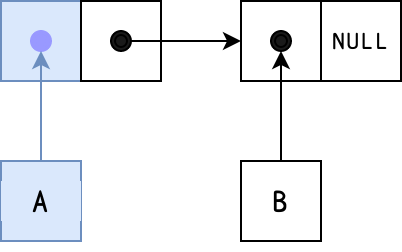
\includegraphics[width=0.3\textwidth]{figures/x1.png}
\caption{The result of car invocation}
\end{figure}

\par \verb|cdr| is used to query a list's tail (\verb|1∘↓|), i.e. everything besides it's head, which is why it's sometimes called \textit{beheading}. \verb|cdr| of a single-element or empty list is \textit{NULL}.

\begin{figure}[H]
\centering
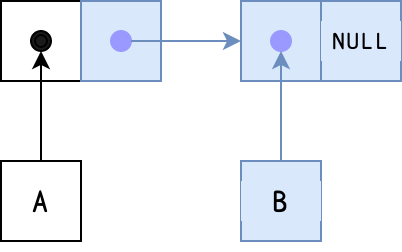
\includegraphics[width=0.3\textwidth]{figures/x2.png}
\caption{The result of car invocation}
\end{figure}

\par \verb|cons| is used to prepend a node (head and a tail) to a list. The tail of the newly created node with given head is set to the provided list. For instance, the list demonstrated in previous examples could be made using \verb|(cons A (cons B null))|. A more concise version of this expression is \verb|(tie A B)|. \verb|tie| behaves like a chain of \verb|cons| invocation, where the last invocation prepends to a \textit{NULL} list. A parallel could be drawn between \verb|cons & tie| and \verb|if & cond|.

\section{Functional list processing}

\par In MalbolgeLISP, the preferred way to process data involves functional devices introduced with MalbolgeLISP v1.2. Most of them were borrowed from Haskell\footnote{\verb|intersperse|, \verb|filter|, \verb|zipwidth|, etc..} and APL\footnote{to name a few: \verb|where|, \verb|take|, \verb|drop|, \verb|map|, \verb|replicate|, \verb|rev|}.

\subsection{iota}

\par The \verb|iota| function exhibits the same behavior as it's C++ counterpart\footnote{\url{https://en.cppreference.com/w/cpp/algorithm/iota}}, although the concept of an index generator has been introduced by APL. \verb|iota| assumes the index origin of 0, so it generates indices in range $[0, n)$. Unlike in APL, \verb|iota| isn't ambivalent nor doesn't support taking a list as it's only argument:

\begin{verbatim}
; MalbolgeLISP
% (iota 5)
.....|...
(0 1 2 3 4)
% (iota '(3 3))
..........|...E030
% (iota '(1 2 3) '(4 5 6))
..................|..E029


      ⍝ APL
      ⎕io←0
      ⍳ 3 3
┌───┬───┬───┐
│0 0│0 1│0 2│
├───┼───┼───┤
│1 0│1 1│1 2│
├───┼───┼───┤
│2 0│2 1│2 2│
└───┴───┴───┘
      ⍳ 5
0 1 2 3 4
      'ABCDEF'⍳'ACF'
0 2 5
\end{verbatim}

\subsection{size}

\par The \verb|size| functions yields the length of a list (in $O(n)$ time complexity). It traverses the list shallowly and doesn't account for it's depth. For instance, a very inefficient identity function on numbers could be implemented to demonstrate it's behavior:

\begin{verbatim}
; MalbolgeLISP
% (def f (atop size iota))
...........|......
bind/syn
% (f 6)
.....|.........
6
% (f 3)
.....|.........
3


      ⍝ APL
      f←≢⍳
      f 6
6
      f 3
3
\end{verbatim}

\subsection{n-th}

\par Picking arbitrary elements from a list is done using \verb|nth|, or a constant $n$-th (the \verb|#| prefix). For example, to pick $n$-th element from the end of a list, the following function might be used:

\begin{verbatim}
; MalbolgeLISP
% (def nl (dyad (nth [(size y) - [x + 1]] y)))
.............................|..
(lambda (x y) (nth (- (size y) (+ x 1)) y))
% (nl '(1 2 3 4 5) 2)
..............|................
3


      ⍝ APL
      nl←⊃⌽
      2 nl 1 2 3 4 5
3
\end{verbatim}

\par \textit{Constant n-th} is an alternative way to query the $n$-th (where $n$ is constant) element of a list. \verb|#N| is equivalent to \verb|(bind nth N)|. \textit{constant n-th} is in many ways similar to a tack - it could even be implemented using a tack and \verb|lift|. For instance:

\begin{verbatim}
; Demonstration of constant n-th
% (print ((atop #1 map) (bind lazy ~) '(0 1 1 1 1 0)))
.............................|................................................
0

0

; Correspondence between constant n-th and tack/lift:
#N <=> (bind lift $N)
\end{verbatim}

\subsection{map}

\par \verb|map| is an ubiquitous higher-order function originating from functional languages present in C++\footnote{\url{https://en.cppreference.com/w/cpp/algorithm/transform}}, APL\footnote{\url{https://help.dyalog.com/latest/index.htm#Language/Primitive\%20Operators/Each\%20with\%20Monadic\%20Operand.htm}} or Java\footnote{\url{https://docs.oracle.com/javase/8/docs/api/java/util/stream/Stream.html#map-java.util.function.Function-}}. \verb|map| is reponsible for transforming (\textit{mapping}) one list into another of equal length, by calling a functor on every element of the original list. It takes any callable first argument, and a list second argument. For example:

\begin{verbatim}
% (map (bind selfie *) (iota 6))
...............|..........................................................
(0 1 4 9 16 25)
% (map ~ '(1 0))
...........|..........
(0 1)
% (map ~ null)
......|....
null
\end{verbatim}

\subsection{filter}

\par \verb|filter| is a higher order function that conditionally removes elements of a list. First, the list is mapped, and then the elements that correspond to falsy values in the list obtained by mapping are removed, and truthy values are kept. \par \verb|filter| behaves in the same way as \verb|map| when the second argument is \textit{NULL}. To demonstrate:

\begin{verbatim}
; MalbolgeLISP
% (filter (bind' % 2) (iota 10))
...............|......................................................
(1 3 5 7 9)
% (filter (bind' % 2) null)
...........|..
null


      ⍝ APL
      filter←{⍵/⍨⍺⍺¨⍵}
      2∘| filter ⍳10
┌→────────┐
│1 3 5 7 9│
└~────────┘
      2∘| filter ⍬
┌⊖┐
│0│
└~┘
\end{verbatim}

\subsection{rev}

\par \verb|rev| is an ambivalent built-in function inspired by APL's \textit{reverse/rotate}\footnote{\url{https://aplwiki.com/wiki/Reverse} and \url{https://aplwiki.com/wiki/Rotate}}. The monadic case simply reverses a list, while the dyadic case rotates it. Since MalbolgeLISP doesn't support rotation with a negative argument, but the dyadic rotation with negative parameter can be defined in an alternative way.

\begin{verbatim}
; MalbolgeLISP
% (rev (iota 5))
.........|.....
(4 3 2 1 0)
% (rev 3 (iota 6))
..........|......
(3 4 5 0 1 2)
% (def rev' (dyad (rev [(size y) - x] y)))
........................|..
(lambda (x y) (rev (- (size y) x) y))
% (rev' 2 (iota 6))
..........|...............
(4 5 0 1 2 3)


      ⍝ APL
      ⌽⍳5
┌→────────┐
│4 3 2 1 0│
└~────────┘
      3⌽⍳6
┌→──────────┐
│3 4 5 0 1 2│
└~──────────┘
      ¯2⌽⍳6
┌→──────────┐
│4 5 0 1 2 3│
└~──────────┘
\end{verbatim}

\subsection{any, every}

\par \verb|any| and \verb|every| are closely tied to each other. \verb|any| returns \verb|1| if its functor returned a truthy value for \textbf{any} element (and \verb|0| otherwise), and \verb|every| returns \verb|1| if its functor returned a truthy value for \textbf{every} element (and \verb|0| otherwise). \verb|any| and \verb|every| short-circuit (otherwise, they would be easy to implement using \verb|filter|). To demonstrate:

\begin{verbatim}
; MalbolgeLISP
% (every (bind = 2) '(2 2 2 2))
..................|................................
1
% (any (bind = 2) '(2 2 2 2))
..................|................................
1
% (every (bind = 3) '(3 3 2))
.................|..............
0
% (any (bind = 3) '(0 1 2))
.................|..............
0


      ⍝ APL
      ⍝ Note: This implementation doesn't short-circuit
      any←{∨/⍺⍺¨⍵}
      every←{∧/⍺⍺¨⍵}
      2∘= every 2 2 2
1
      2∘= any 1 2 3
1
      3∘= every 3 3 2
0
      3∘= any 1 2 2
0
\end{verbatim}

\subsection{zip, zipwith}

\par \verb|zip| juxtaposes elements from two lists to form a list of pairs of corresponding elements from them. The pairs can be further processed to produce a flat result if \verb|zipwith| is used. \verb|zip| and \verb|zipwith| will return a list of size \verb|⌊⍥≢|\footnote{when end of list is encountered when the pairs are formed, the operation finishes}.

\begin{verbatim}
; MalbolgeLISP
% [zip selfie (iota 3)]
..........|..........
((0 0) (1 1) (2 2))
% [+ zipwith (iota 3) (iota 3)]
...............|.....................
(0 2 4)


      ⍝ APL
      zip←,¨
      zipwith←{⍺⍺/¨⍺,¨⍵}
      zip⍨ ⍳3
┌→──────────────────┐
│ ┌→──┐ ┌→──┐ ┌→──┐ │
│ │0 0│ │1 1│ │2 2│ │
│ └~──┘ └~──┘ └~──┘ │
└∊──────────────────┘
      (⍳ 3) (+ zipwith) (⍳ 3)
┌→────┐
│0 2 4│
└~────┘
\end{verbatim}

\subsection{flatten, flatmap}

\par \verb|flatten| and \verb|flatmap|'s mutual relations somewhat resemble \verb|zip| and \verb|zipwith|. While the first operation is a function that simply flattens a list, the second function is a \verb|map| which result is flattened afterwards. List flattening isn't deep:

\begin{verbatim}
; MalbolgeLISP
% (flatten '((1 2) (3 4)))
..................|...
(1 2 3 4)
% (flatten '(((1 2) (3 4)) (3 4)))
..........................|...
((1 2) (3 4) 3 4)
; Simple deep flattening
% (def deepf (bind iterate = flatten))
............|........
bind/syn
% (deepf '(((1 2) (3 4)) (3 4)))
..........................|............................
(1 2 3 4 3 4)
; Successor and predecessor of a number
% (def sp (monad (tie [x + 1] [x - 1])))
.........................|..
(lambda (x) (tie (+ x 1) (- x 1)))
% (flatmap sp '(1 2 3 4))
.............|........................................................
(2 0 3 1 4 2 5 3)
; As opposed to...
% (map sp '(1 2 3 4))
.............|........................................................
((2 0) (3 1) (4 2) (5 3))

      ⍝ APL
      f←⊃,/
      f ((1 2) (3 4))
1 2 3 4
      f (((1 2) (3 4)) (3 4))
┌───┬───┬─┬─┐
│1 2│3 4│3│4│
└───┴───┴─┴─┘
      ⍝ two choices for deep flattening
      ⍝ MalbolgeLISP port:
      g←f⍣≡
      ⍝ Idiomatic APL:
      h←∊
      g (((1 2) (3 4)) (3 4))
1 2 3 4 3 4
      h (((1 2) (3 4)) (3 4))
1 2 3 4 3 4
      sp←(+,-)∘1
      fm←{⊃,/⍺⍺¨⍵}
      sp fm 1 2 3 4
2 0 3 1 4 2 5 3
      sp¨ 1 2 3 4
┌───┬───┬───┬───┐
│2 0│3 1│4 2│5 3│
└───┴───┴───┴───┘
\end{verbatim}

Illustratively, flattening a list alters it in the following way:

\begin{figure}[H]
\centering
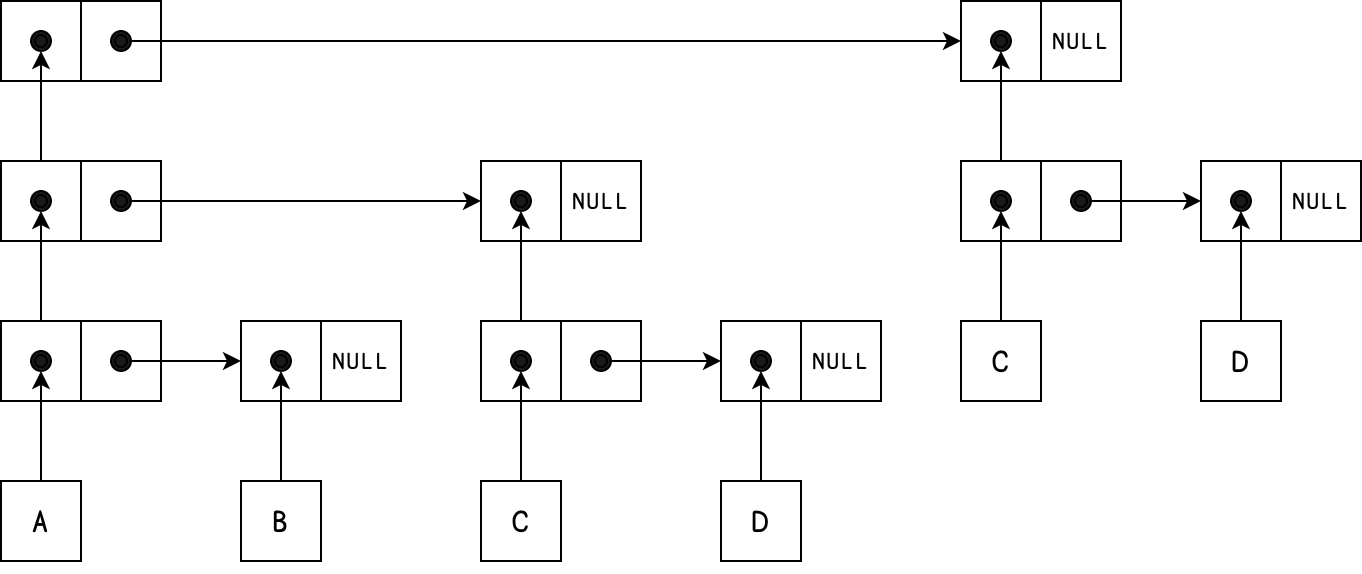
\includegraphics[width=\textwidth]{figures/beforeFlatten.png}
\caption{A list before flattening}
\end{figure}

\begin{figure}[H]
\centering
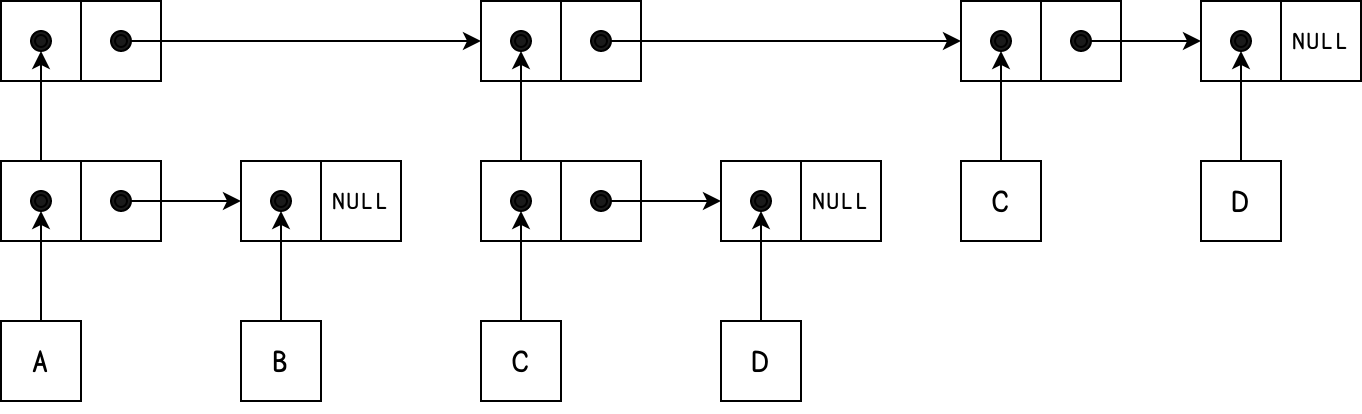
\includegraphics[width=\textwidth]{figures/afterFlattening.png}
\caption{A list after flattening}
\end{figure}

\subsection{folds}

\par Folding is a way to transform an entire list by putting a binary operation between each element of it. Since folding must yield a result, and the list might be empty, \verb|fold| takes an additional argument which specifies the identity element, which semantically means that the value is left unchanged\footnote{for instance, the identity element of $+$ is \verb|0|, since $x + 0 = x$ and the identity element of $\times$ is \verb|1|, since $x \times 1 = x$}. Since APL supports only reductions, the comparison between MalbolgeLISP and APL is not demonstrated in this example.

\begin{verbatim}
% (fold 0 + '(1 2 3 4 5))
...............|.........................
15
% [[[[[0 + 1] + 2] + 3] + 4] + 5]
..........................|................
15
% (fold 0 + null)
.......|.....
0
\end{verbatim}

\par If it is known that the list contains at least one element, \verb|fold'| can be used, which is equivalent to APL's reductions:

\begin{verbatim}
; MalbolgeLISP
% (fold' + '(1 2 3 4 5))
...............|.........................
15


      ⍝ APL
      +/ 1 2 3 4 5
15
\end{verbatim}

\subsection{where}

\par \verb|where| is a function borrowed from APL - \verb|⍸|\footnote{\url{http://help.dyalog.com/16.0/Content/Language/Primitive\%20Functions/Where.htm}}. It returns the indices on which the input array contains truthy values. If the truthy value is greater than one, it's repeated that amount of times. For example:

\begin{verbatim}
; MalbolgeLISP
% (where '(1 0 1 0 1 1 1 0))
................|...
(0 2 4 5 6)
% (where '(1 2 3 4))
............|...
(0 1 1 2 2 2 3 3 3 3)


      ⍝ APL
      ⍸1 0 1 0 1 1 1 0
0 2 4 5 6
      ⍸1 2 3 4
0 1 1 2 2 2 3 3 3 3
\end{verbatim}

\subsection{count}

\par \verb|count| counts the amount of times it's functor returned a truthy value for each element of a list. It can be trivially expressed as a \verb|fold| and \verb|map|. An example of \verb|count| usage follows.

\begin{verbatim}
; MalbolgeLISP
% (count (bind = 2) '(2 2 3 2 2 3))
....................|............................................
4
% (def count' (dyad (fold 0 + (map [[< bind 0] atop x] y))))
...............................|..
(lambda (x y) (fold 0 + (map (atop (bind < 0) x) y)))
% (count' (bind = 2) '(2 3 2 3))
..................|..............................................
..........................................................
2


      ⍝ APL
      count←{+/(0<⍺⍺)¨⍵}
      2∘= count 2 3 2 3 2 2
4
\end{verbatim}

\subsection{replicate}

\par \verb|replicate| is one of the most overloaded functions in MalbolgeLISP. It takes three different forms depending on the argument types:
\begin{itemize}
    \item \verb|replicate list list| - copy elements from list 2 according to the masks in list 1. comparable to \verb|filter|\footnote{a filter-like function is implemented in APL using replicate}, but it takes a pre-mapped array instead of a functor.
    \item \verb|replicate num list| - duplicate the list specified amount of times
    \item \verb|replicate num any| - make a list out of any atom repeated specified amount of times
\end{itemize}

\begin{verbatim}
; MalbolgeLISP
% (replicate 5 hello)
......|....
(hello hello hello hello hello)
% (replicate 5 '(1 2))
...........|....
(1 2 1 2 1 2 1 2 1 2)
% (replicate '(1 0 2) '(1 2 3))
..................|....
(1 3 3)


      ⍝ APL
      replicate1←⍴∘⊂
      5 replicate1 'hello'
┌─────┬─────┬─────┬─────┬─────┐
│hello│hello│hello│hello│hello│
└─────┴─────┴─────┴─────┴─────┘
      replicate2←{↑,/⍺⍴⊂⍵}
      5 replicate2 1 2
1 2 1 2 1 2 1 2 1 2
      1 0 2/1 2 3
1 3 3
\end{verbatim}

\subsection{scan}

\par \verb|scan| performs a \verb|fold| with partial results. The standard behavior diverges from APL (since the identity element is excluded), but it can be accomplished using \verb|scan'|, which assumes that the input list has at least a single element.

\begin{verbatim}
; MalbolgeLISP
% (scan' * '(1 2 3 4 5))
..............|....................
(1 2 6 24 120)
% (scan * 1 '(1 2 3 4 5))
..............|........................
(1 1 2 6 24 120)


      ⍝ APL
      ×\1 2 3 4 5
1 2 6 24 120
\end{verbatim}

\subsection{uniq}

\par \verb|uniq| returns unique elements of a list using the \textit{formal definition of equality}. It uses an algorithm which makes $O(n^2)$ equality checks in the pessimistic case. To demonstrate:

\begin{verbatim}
; MalbolgeLISP
% (uniq '(1 6 2 5 2 6 2 3))
................|...
(1 6 2 5 3)
% (uniq '((1 2) (1 2) (1 2 3) (4 5) 6 (4 5)))
...................................|...
((1 2) (1 2 3) (4 5) 6)

      ⍝ APL
      ∪ 1 6 2 5 2 5 6 2 3
1 6 2 5 3
      ∪ ((1 2) (1 2) (1 2 3) (4 5) 6 (4 5))
┌───┬─────┬───┬─┐
│1 2│1 2 3│4 5│6│
└───┴─────┴───┴─┘
\end{verbatim}

\subsection{sort}

\par \verb|sort| is a function that sorts a list with an arbitrary comparator (or assumes a default comparator for sorting numeric lists, if none was provided). MalbolgeLISP utilises the insertion sort algorithm\footnote{because of it's simplicity and performance on small lists, which are going to realistically be the main use case for it in MalbolgeLISP}. It has a time complexity of $O(n^2)$ and auxiliary space requirement of $O(1)$. It takes maximum time to sort a list if elements are sorted in reverse order, and it takes minimum time when the elements are already sorted. For example:

\begin{verbatim}
; MalbolgeLISP
% (sort '(1 9 5 8 2 3 9 5))
................|...
(1 2 3 5 5 8 9 9)
% (sort '(1 9 5 8 2 3 9 5))
................|...
(1 2 3 5 5 8 9 9)
% (sort > '(1 9 5 8 2 3 9 5))
.................|......................................
........................................................
......................
(1 2 3 5 5 8 9 9)


      ⍝ APL
      ⍝ Implementation of an insertion sort.
      sortn←((≥⊢⍤/⊢),⊣,<⊢⍤/⊢)/
      sortn 32 4 1 34 95 3 2 120 ¯38
┌────────────────────────┐
│¯38 1 2 3 4 32 34 95 120│
└────────────────────────┘
      ⍝ A more idiomatic way of solving the problem:
      sortn1←{⍵[⍋⍵]}
      sortn1 32 4 1 34 95 3 2 120 ¯38
¯38 1 2 3 4 32 34 95 120
      ⍝ Sorting with a comparator
      sortc←{p←⍺⍺⋄{r←/∘⍵⋄c←⍺p⍵⋄(r c),⍺,r ~c}/⍵}
      > sortc 32 4 1 34 95 3 2 120 ¯38
┌────────────────────────┐
│¯38 1 2 3 4 32 34 95 120│
└────────────────────────┘
\end{verbatim}

\subsection{take, take', drop, drop'}

\par \verb|take| and \verb|take'| extract $n$ elements from the front (\verb|take|) or from the back (\verb|take'|) of a list. They correspond to \verb|↑| and \verb|((-⊣)↑⊢)| in APL. \verb|take| triggers a copy, while \verb|take'| doesn't:

\begin{figure}[H]
\centering
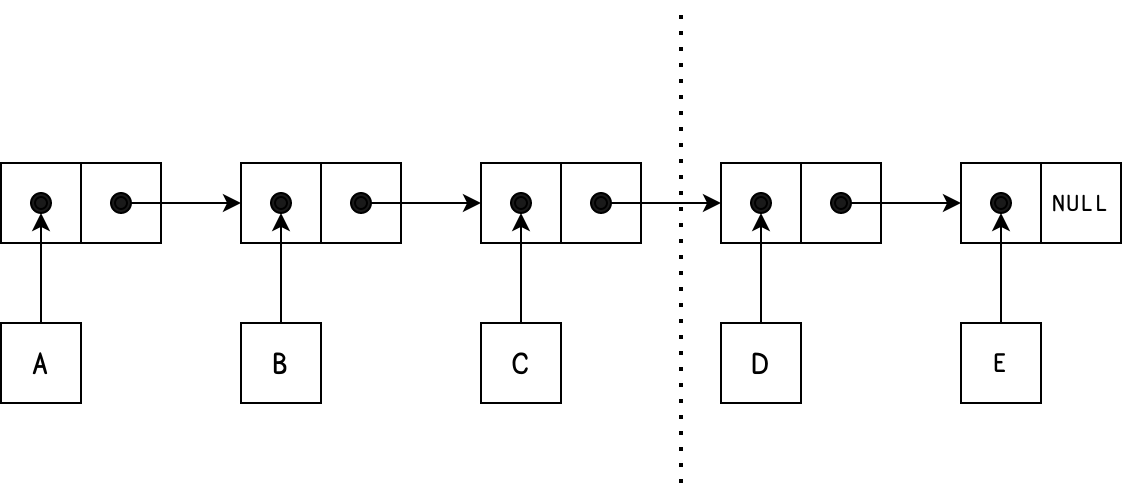
\includegraphics[width=0.8\textwidth]{figures/take.png}
\caption{Taking the first three elements from a list}
\end{figure}

\par The list must be cloned, since setting the tail of the list node which holds \verb|C| to \textit{NULL} (to yield a new list) would invalidate existing references. This doesn't apply to \verb|take'|, since it doesn't have to modify the memory it's operating on.

\begin{verbatim}
; MalbolgeLISP
% (take 3 '(1 2 3 4 5))
..............|....
(1 2 3)
% (take' 3 '(1 2 3 4 5))
..............|....
(3 4 5)


      ⍝ APL
      3↑1 2 3 4 5
1 2 3
      ¯3↑1 2 3 4 5
3 4 5
\end{verbatim}

\par \verb|drop| and \verb|drop'| exhibit the same behavior. They drop $n$ elements from the front (\verb|drop|) or the back (\verb|drop'|) of a list. Dropping elements from the back requires a copy, while dropping them from the front does, for the reasons outlined above.

\begin{verbatim}
; MalbolgeLISP
% (drop 3 '(1 2 3 4 5))
..............|....
(4 5)
% (drop' 3 '(1 2 3 4 5))
..............|....
(1 2)


      ⍝ APL
      3↓1 2 3 4 5
4 5
      ¯3↓1 2 3 4 5
1 2
\end{verbatim}

\section{Iteration and recursion}

\par This section is intended to demonstrate various implementations of the Fibonacci series in MalbolgeLISP\footnote{in comparison to APL} using iteration and recursion. Then, the approaches will be judged by cleaniness, conciseness and performance.

\par The naive, doubly recursive attempt timed at 1m 19s follows:

\begin{minted}{lisp}
(defun fib1 (n) (
    if [n < 2]
        n
        [(fib1 [n - 1]) + (fib1 [n - 2])]))
(fib1 6) ; => 8
; APL: {1≥⍵:⍵ ⋄ (∇⍵-2)+∇⍵-1} 6
\end{minted}

\par A singly-recursive attempt which keeps track of the accumulator tuple. There exist two versions of it - a port of the APL solution and the idiomatic MalbolgeLISP attempt, which is much faster than the port, since it takes advantage of MalbolgeLISP's support of functions of arity 3 or higher.

\begin{minted}{lisp}
; APL version: {⍺←0 1 ⋄ 0=⍵:⊃⍺ ⋄ (1↓⍺,+/⍺)∇⍵-1} 6
; Direct port at 1m 6s:
(defun fib2 (n) ((lambda (a w) (
    if [w = 0]
        (#0 a)
        ((bruijn 0) (tie (#1 a) (lift + a)) [w - 1]))) '(0 1) n))
; A more idiomatic solution at 54s:
(defun fib2 (n) ((lambda (x y w) (
    if [w = 0]
        x
        ((bruijn 0) y [x + y] [w - 1]))) 0 1 n))
\end{minted}

\par An iterative attempt timed at 43s:

\begin{minted}{lisp}
; APL version: {⊃+\∘⌽⍣⍵⍳2} 6
(defun fib3 (n) (#0 (
    iterateN n (lambda (x) (
        tie (#1 x) [(#0 x) + (#1 x)])) '(0 1))))
\end{minted}

\par It should be noted that even though the second approach is generally faster, it's not as clean as the first or third one. The first approach is the slowest, while the second and third approaches are faster. Generally, the most concise, clean and the fastest attempt is the iterative attempt.
